%!TEX TS-program = xelatex

% Author: Georgy Perevozchikov (gosha20777@live.com)
% https://github.com/gosha20777/bachelor-diploma

\documentclass[a4paper,14pt]{extarticle} % 14й шрифт
%%% Преамбула %%%

\usepackage{fontspec} % XeTeX
\usepackage{xunicode} % Unicode для XeTeX
\usepackage{xltxtra}  % Верхние и нижние индексы
\usepackage{pdfpages} % Вставка PDF

\usepackage{listings} % Оформление исходного кода
\lstset{
    basicstyle=\small\ttfamily, % Размер и тип шрифта
    breaklines=true, % Перенос строк
    tabsize=2, % Размер табуляции
    literate={--}{{-{}-}}2 % Корректно отображать двойной дефис
}

% Шрифты, xelatex
\defaultfontfeatures{Ligatures=TeX}
\setmainfont{Times New Roman} % Нормоконтроллеры хотят именно его
\newfontfamily\cyrillicfont{Times New Roman}
%\setsansfont{Liberation Sans} % Тут я его не использую, но если пригодится
\setmonofont{FreeMono} % Моноширинный шрифт для оформления кода

% Русский язык
\usepackage{polyglossia}
\setdefaultlanguage{russian}

\usepackage{amssymb,amsfonts,amsmath} % Математика
\numberwithin{equation}{section} % Формула вида секция.номер

\usepackage{enumerate} % Тонкая настройка списков
\usepackage{indentfirst} % Красная строка после заголовка
\usepackage{float} % Расширенное управление плавающими объектами
\usepackage{multirow} % Сложные таблицы

% Пути к каталогам с изображениями
\usepackage{graphicx} % Вставка картинок и дополнений
\graphicspath{{images/}{images/userguide/}{images/testing/}{images/infrastructure/}{extra/}{extra/drafts/}}

% Формат подрисуночных записей
\usepackage{chngcntr}
\counterwithin{figure}{section}

% Гиперссылки
\usepackage{hyperref}
\hypersetup{
    colorlinks, urlcolor={black}, % Все ссылки черного цвета, кликабельные
    linkcolor={black}, citecolor={black}, filecolor={black},
    pdfauthor={Георгий Перевозчиков},
    pdftitle={Разработка моделей глубокого машинного обучения для распознования людей по аэрофотоснимкам в Поисково-Спасательных Операциях}
}

% Оформление библиографии и подрисуночных записей через точку
\makeatletter
\renewcommand*{\@biblabel}[1]{\hfill#1.}
\renewcommand*\l@section{\@dottedtocline{1}{1em}{1em}}
\renewcommand{\thefigure}{\thesection.\arabic{figure}} % Формат рисунка секция.номер
\renewcommand{\thetable}{\thesection.\arabic{table}} % Формат таблицы секция.номер
\def\redeflsection{\def\l@section{\@dottedtocline{1}{0em}{10em}}}
\makeatother

\renewcommand{\baselinestretch}{1.4} % Полуторный межстрочный интервал
\parindent 1.27cm % Абзацный отступ

\sloppy             % Избавляемся от переполнений
\hyphenpenalty=1000 % Частота переносов
\clubpenalty=10000  % Запрещаем разрыв страницы после первой строки абзаца
\widowpenalty=10000 % Запрещаем разрыв страницы после последней строки абзаца

% Отступы у страниц
\usepackage{geometry}
\geometry{left=3cm}
\geometry{right=1cm}
\geometry{top=2cm}
\geometry{bottom=2cm}

% Списки
\usepackage{enumitem}
\setlist[enumerate,itemize]{leftmargin=12.7mm} % Отступы в списках

\makeatletter
    \AddEnumerateCounter{\asbuk}{\@asbuk}{м)}
\makeatother
\setlist{nolistsep} % Нет отступов между пунктами списка
\renewcommand{\labelitemi}{--} % Маркет списка --
\renewcommand{\labelenumi}{\asbuk{enumi})} % Список второго уровня
\renewcommand{\labelenumii}{\arabic{enumii})} % Список третьего уровня

% Содержание
\usepackage{tocloft}
\renewcommand{\cfttoctitlefont}{\hspace{0.38\textwidth}\MakeTextUppercase} % СОДЕРЖАНИЕ
\renewcommand{\cftsecfont}{\hspace{0pt}}            % Имена секций в содержании не жирным шрифтом
\renewcommand\cftsecleader{\cftdotfill{\cftdotsep}} % Точки для секций в содержании
\renewcommand\cftsecpagefont{\mdseries}             % Номера страниц не жирные
\setcounter{tocdepth}{3}                            % Глубина оглавления, до subsubsection

% Нумерация страниц справа сверху
\usepackage{fancyhdr}
\pagestyle{fancy}
\fancyhf{}
\fancyhead[R]{\textrm{\thepage}}
\fancyheadoffset{0mm}
\fancyfootoffset{0mm}
\setlength{\headheight}{17pt}
\renewcommand{\headrulewidth}{0pt}
\renewcommand{\footrulewidth}{0pt}
\fancypagestyle{plain}{ 
    \fancyhf{}
    \rhead{\thepage}
}

% Формат подрисуночных надписей
\RequirePackage{caption}
\DeclareCaptionLabelSeparator{defffis}{ -- } % Разделитель
\captionsetup[figure]{justification=centering, labelsep=defffis, format=plain} % Подпись рисунка по центру
\captionsetup[table]{justification=raggedright, labelsep=defffis, format=plain, singlelinecheck=false} % Подпись таблицы слева
\addto\captionsrussian{\renewcommand{\figurename}{Рис.}} % Имя фигуры

% Пользовательские функции
\newcommand{\addimg}[4]{ % Добавление одного рисунка
    \begin{figure}
        \centering
        \includegraphics[width=#2\linewidth]{#1}
        \caption{#3} \label{#4}
    \end{figure}
}
\newcommand{\addimghere}[4]{ % Добавить рисунок непосредственно в это место
    \begin{figure}[H]
        \centering
        \includegraphics[width=#2\linewidth]{#1}
        \caption{#3} \label{#4}
    \end{figure}
}
\newcommand{\addtwoimghere}[5]{ % Вставка двух рисунков
    \begin{figure}[H]
        \centering
        \includegraphics[width=#2\linewidth]{#1}
        \hfill
        \includegraphics[width=#3\linewidth]{#2}
        \caption{#4} \label{#5}
    \end{figure}
}
\newcommand{\addimgapp}[2]{ % Это костыль для приложения Б
    \begin{figure}[H]
        \centering
        \includegraphics[width=1\linewidth]{#1}
        \caption*{#2}
    \end{figure}
}

% Заголовки секций в оглавлении в верхнем регистре
\usepackage{textcase}
\makeatletter
\let\oldcontentsline\contentsline
\def\contentsline#1#2{
    \expandafter\ifx\csname l@#1\endcsname\l@section
        \expandafter\@firstoftwo
    \else
        \expandafter\@secondoftwo
    \fi
    {\oldcontentsline{#1}{\MakeTextUppercase{#2}}}
    {\oldcontentsline{#1}{#2}}
}
\makeatother

% Оформление заголовков
\usepackage[compact,explicit]{titlesec}
\titleformat{\section}{}{}{12.5mm}{\centering{\thesection\quad\MakeTextUppercase{#1}}\vspace{1.5em}}
\titleformat{\subsection}[block]{\vspace{1em}}{}{12.5mm}{\thesubsection\quad#1\vspace{1em}}
\titleformat{\subsubsection}[block]{\vspace{1em}\normalsize}{}{12.5mm}{\thesubsubsection\quad#1\vspace{1em}}
\titleformat{\paragraph}[block]{\normalsize}{}{12.5mm}{\MakeTextUppercase{#1}}

% Секции без номеров (введение, заключение...), вместо section*{}
\newcommand{\anonsection}[1]{
    \phantomsection % Корректный переход по ссылкам в содержании
    \paragraph{\centerline{{#1}}\vspace{1.5em}}
    \addcontentsline{toc}{section}{\uppercase{#1}}
}

% Секции для приложений
\newcommand{\appsection}[1]{
    \phantomsection
    \paragraph{\centerline{{#1}}}
    \addcontentsline{toc}{section}{\uppercase{#1}}
}

% Библиография: отступы и межстрочный интервал
\makeatletter
\renewenvironment{thebibliography}[1]
    {\section*{\refname}
        \list{\@biblabel{\@arabic\c@enumiv}}
           {\settowidth\labelwidth{\@biblabel{#1}}
            \leftmargin\labelsep
            \itemindent 16.7mm
            \@openbib@code
            \usecounter{enumiv}
            \let\p@enumiv\@empty
            \renewcommand\theenumiv{\@arabic\c@enumiv}
        }
        \setlength{\itemsep}{0pt}
    }
\makeatother

\setcounter{page}{4} % Начало нумерации страниц
 % Подключаем преамбулу

%%% Начало документа
\begin{document}

%\includepdf{pz} % Пояснительная записка
%\includepdf[pages={1,2}]{task} % Задание на диплом печатается на одном листе с двух сторон
%помимо ПЗ и задания, в диплом также вкладывается отзыв руководителя и рецензия

\tableofcontents % Содержание 
%\clearpage

\anonsection{Введение}

В XXI веке роль технологий обучения и AI (англ. artificial intelligence -- искуственный интеллект) трудно переоценить. Благодоря им значительно упрощается обработка больших данных, люди могут предсказывать события, автоматизировать рпроизводственные процессы, делать новые научне открытия, и решают множество других задач и решать другие важные для человека задачи.

Одной из областей машинного обучения яаляется CV (англ. Compurer Vision -- компьютерное зение). CV позволяет обрабатывать с помощью сверточных нейронных сетей изображения или видео и на основе их анализа делать различные заключения. Благодоря этой технологии время необходимое на обработку таких данных значительно сокращается а человек избавляется от выполнения рутиной работы. Также невилируется фактор усталости человека при выполнении ручной обработки данных, что зачастую приводит к повышению качества выполнения задачи.

Отдельной областью применения является поиск пропавших или потерявшихся людей в природной зоне. В воследнее время для анализа местности все чаще применяются БПЛА (Беспилотные Летательные Аппараты) для проведения аэрофотосъемки. Процесс анализа таких изображений довольно трудоемкий для человека, по этому его можно автоматизировать с помощью технологий компьютерного зрания (CV). 

В описанном в данной работе исследовании приводится мехонизм решения описаной выше проблемы с применением современных технологий компьютерного зрения. Использование сверточных нейронных сетей сопсобно в короткие сроки решить задачу детектирования и локализации пропаышего человека на местности, что нередко может спасти ему жизнь. 

Цель работы -- исследование и разаработка различных архитектур СНС (сверточных нейронных сетей) решающих задачу детектирования потерявшихся в лесу людей по аэрофотоснимкам полученных с БПЛА, разработка пользовательского ПО (Программного Обеспечения) реализующего данную технологию с целью возможного внедрения в ПСО (поисково-спасательные отряды) для непосредственного применения. В разделе 1 описывается проблемы поиска пропаыших в лесу людей и их детектирования по аэрофотоснимкам. В резделе 2 описаны современные методы анализа изображений, принципы работы сверточных нейронных сетей и метрики их оценивания. В разделе 3 изложен процесс обора и подготовки данных для обучения нейросетевых алгоритмов. В разделе 4 производится сравнение раздичных архитектур СНС и объясняется выбор архитектуры RetinaNet-Resnet50. В разделе 5 приводится подробное описание архитектуры RetinaNet-Resnet50. В разделе 6 описан процесс обучения RetinaNet-Resnet50, исследования, улучшающие качество распознования (FPN-shift и Deep FPN), и приведены результаты экспериментов. В разделе 7 приведено пользовательского ПО. В разделе 8 приведены результаты использования данного ПО в различных ПСО.
\clearpage % Введение
\section{Проблема поиска пропавших людей}\label{sect-1}

Неподготовленный человек, попавший в природную среду, может легко заблудиться и пропасть. Достаточно часто люди уходят на природу, в лес -- за грибами, с прогулочными или иными целями -- теряют ориентиры, после чего самостоятельно выбраться из природных условий становится проблематично.

Розыском таких пропавших людей занимаются как и государственные структуры (МЧС, полиция), так и волонтёры в составе Поисково-Спасательных Отрядов (ПСО). Так, например, в России наиболее известными ПСО являются "Лиза Алерт", "Экстремум", "Сова", "Запад", "Орен Спас". Подобные организации распространены и в других странах по всему миру.

Так, по приблизительным оценкам в России каждый год пропадает более ста двадцати тысяч человек, в США -- более ста тысяч, на территории стран Европейского Союза эта цифра составляет приблизительно девяноста тысяч человек.

\subsection{Основные факторы риска потерявшегося человека в природной зоне}

Положение потерявшегося человека часто усугубляется из-за физических и психологических факторов, таких как:

\begin{itemize}
    \item Обезвоживание. Отсутствие доступа к питьевой воде или ограниченный её запас резко снижает возможность человека поддерживать своё стабильное состояние на протяжении длительного времени, которое может потребоваться на проведение спасательной операции;
    \item Гипотермия (переохлаждение). Зимой и в ночное время температура окружающей среды снижается (особенно в природных условиях), а у потерявшегося человека, как правило, нет возможности согреться (если нет соответствующего снаряжения). Данная причина является одной из наиболее частых причин гибели потерявшихся людей;
    \item Травмаы. Человек, который потерялся на природе, нередко начинает паниковать, что приводит к необдуманным, импульсивным поступкам, которые нередко приводят к травмам, после получения которых шансы самостоятельно добраться до цивилизации драматически уменьшаются;
    \item Паника. Осознание потерявшимся факта невозможности самостоятельно выбраться из локации нередко приводит к панике, что резко снижает вероятность успешного выхода потерявшегося человека к цивилизации.
\end{itemize}

Эти и многие другие факторы резко снижают время выживания потерявшегося человека в лесу, что в свою очередь повышает требования к временному ресурсу для поисково-спасательных операций. В среднем потерявшейся человек может продержаться в лесу в течении 6-8 дней, летом и 2-4 дней зимой. Стоит также учесть, что поиск человека может начаться не сразу, а спустя какое-то время. Иными словами -- часто счет идет на часы.
\subsubsection{Основные методики поиска пропавших людей}

Наиболее распространенным способом поиска потерявшегося человека в природной локации является наземная поисковая операция. Это, как правило, пеший поиск с участием ответственных за подобные мероприятия служб или силами волонтёров. 

Район поиска делится на квадраты размером 500$\times$500 метров, и прочесывается отрядом спасателей по заранее оговоренному маршруту (как правило цепью), с целью постараться увидеть или получить отклик потерявшегося человека. 

Данный способ поиска является несомненно точным, но достаточно тяжелым -- необходимо большое количество подготовленных к задаче поиска людей, необходима организация поисковых групп, необходимо выполнение многих других смежных задач. Помимо прочего, пеший поиск является достаточно медленным. Поисковый квадрат размером в лесной зоне закрывается пешей поисковой группой в среднем за 3-6 часов (а таких квадратов может быть несколько).

Другим способом поиска является поиск по фотографиям, с полученных с БПЛА. В последнее время появились небольшие БПЛА и их все чаще применяют спасатели для проведения поисковых работ. 

Над районом поиска составляется маршрут, по которому затем пролетает летательный аппарат, в заранее заданных точках делает фотографии с гео-меткой. После выполнения полётного задания БПЛА возвращается в поисковый штаб, где его оператор меняет на нём аккумулятор и карту памяти со снимками, после чего, загружает следующее полётное задание и дрон отправляется на дальнейшие съёмки с воздуха.

Опытным путём было установлено, что наиболее оптимальная высота для осуществления аэрофотосъёмки региона поиска приблизительно 50 метров. Данная отметка выше крон деревьев, при этом позволяет получить достаточно чёткие фотоснимки, на которых можно заметить человека.

С одной поисковой операции в среднем набирается около четырех тысяч фотографий. Полученные фотографии анализируются специалистами из ГПА (группа просмотра и анализа) с целью найти на них человека. Человек на такой фотографии может быть частично закрыт растительностью и занимает очень мало места -- в среднем взрослый лежачий человек имеет 100 пикселей в высоту и 30 в ширину при исходном размере изображения 4000$\times$3000 пикселей. Это усложняет ручной анализ изображений и пагубно сказывается на усталости анализирующего человека. В среднем опытный специалист из ГПА тратит на анализ одной фотографии около минуты, а его концентрации внимания хватает на анализ 50-70 снимков, после чего, человеку необходим отдых. На анализ четырех тысяч фотографий (одна поисковая операция) у ГПА из 5-6 человек тратится около 6.5 часов.
\subsubsection{Постановка задачи}

Цель работы заключается в исследовании и разработке различных архитектур СНС, решающих задачу детектирования потерявшихся в лесу людей по аэрофотоснимкам полученных с БПЛА, разработке пользовательского ПО, реализующего данную технологию, с целью возможного внедрения в ПСО для непосредственного применения.

В исследовании ведется учет следующих критериев:
\begin{itemize}
    \item Точность алгоритма распознавания -- СНС должна точно находить людей, не пропускать их, а число ложных срабатываний должно быть минимальным;
    \item Скорость алгоритма распознавания -- СНС должна быстро анализировать снимки на персональных компьютерах;
    \item Потребление памяти -- количество потребляемой памяти (зависит от числа параметров СНС и количества ее слоев) должно позволять запускать СНС на персональных компьютерах.
\end{itemize}

Для реализации поставленной цели были сформулированы следующие задачи:
\begin{itemize}
    \item Сбор, анализ и подготовка исходных данных необходимых для обучения нейросетевых математических моделей;
    \item Выбор оптимальной архитектуры нейросетевой модели, проверка возможности ее улучшения, обучение модели;
    \item Проведение оптимизационных работ с целью уменьшение времени работы выбранного нейросетевого алгоритма на ЭВМ;
    \item Разработка интерфейса пользователя;
\end{itemize}

\clearpage % Постановка задачи
\section{Сверточные нейронные сети для решения основных задач компьютерного зрения}

Сверточные нейронные сети (СНС) -- открытые Яном ЛеКуном -- сейчас широко применяются в широком спектре задач анализа изображений. Успех обусловлен возможностью учета двумерной топологии изображения и устойчивости к различным искажениям изображения (изменениям масштаба и кантрастности, смещениям, поворотам и т.д.) в отличие от многослойного персептрона.

На данный момент сверточная нейронная сеть и ее модификации стремительно развиваются и считаются лучшими по точности и скорости алгоритмами нахождения объектов на сцене. Начиная с 2012 года, нейросети занимают первые места на известном международном конкурсе по распознаванию образов ImageNet, во многом обгоняя человека.
\addimghere{2-imagenet-statistics}{1}{Статистика ошибок, совершенных в процессе анализа данных ImageNet за 2010—2015}{imagenet-stat}

dd

\clearpage % Постановка задачи
\section{Сбор и подготовка данных}

Для решения поставленной задачи первоначально был проведен опрос операторов БПЛА из ПСО "Лиза Алерт", и получены несколько примеров снимков. В результате были выяснены следующие аспекты:

\begin{itemize}
    \item Условия съемки:
    \begin{itemize}
        \item Высота -- 40-50 метров над поверхностью земли;
        \item Съемка производиться вертикально (вид сверху);
        \item Во время съемки БПЛА зависает над сценой, чтобы сфокусироваться;
    \end{itemize}
    \item Позы, в которых чаще всего находят потерявшихся людей:
    \begin{itemize}
        \item Стоящий человек (идущий, бегущий);
        \item Сидячий человек (на корточках);
        \item Лежачий человек (на спине);
        \item Лежачий человек (на животе);
        \item Лежачий человек (на боку);
        \item Лежачий в позе эмбриона человек.
    \end{itemize}
\end{itemize}

При поиске доступных открытых решений удалось найти 2 набора данных (dataset-а): SDD (Stanford Drone Dataset) \cite{lib-sdd} и VisDrone DET dataset \cite{lib-visdrone}, но ни один из них не подходил для решения поставленной задачи (рис. \ref{sdd-visdrone-example}). В этих наборах данных несколько отличались условия съемки, а также, отсутствовали, как природная среда, так и интересующие нас позы. Однако, у них есть одно существенное преимущество -- они открыты и довольно распространены, а также, по схожести задачи они значительно ближе, чем какие-либо другие наборы данных. По этому, в описанных ниже исследованиях они использовались для предобучения моделей (а как следствие и сужения доменной области) и оценки качества моделей \cite{lib-transfer-learning}. Также, открытость этих данных и их известность позволила сравнивать качество полученных моделей с уже имеющимися.

\begin{figure}[H]
    \centering
    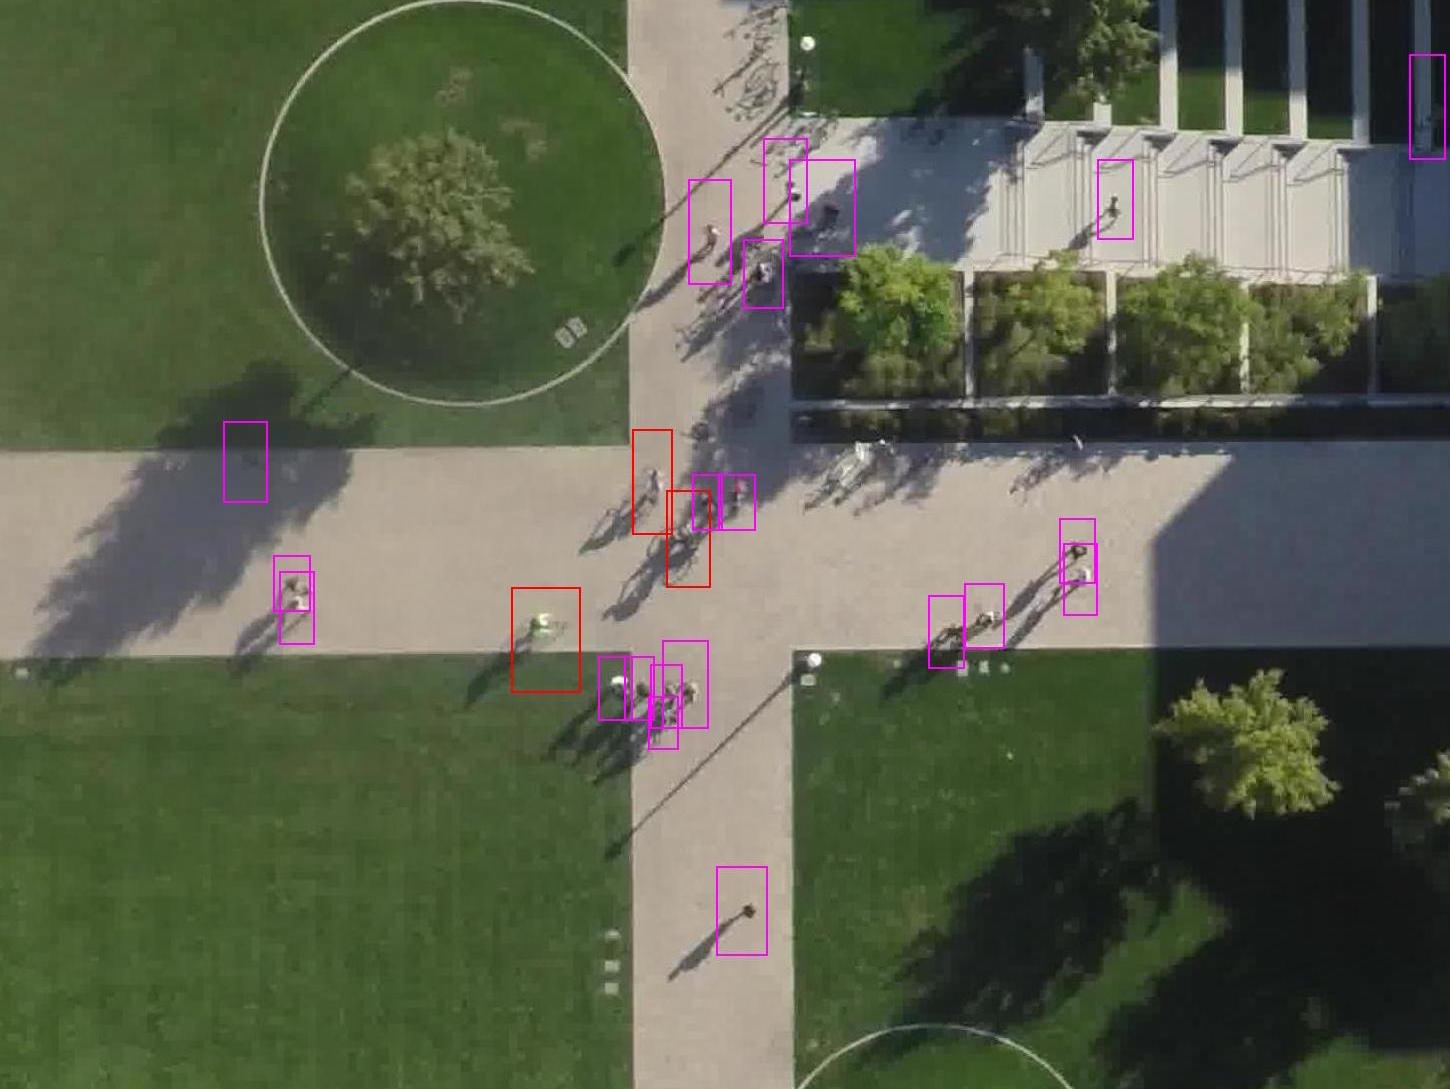
\includegraphics[width=0.42\linewidth]{3-sdd-example}
    \hfill
    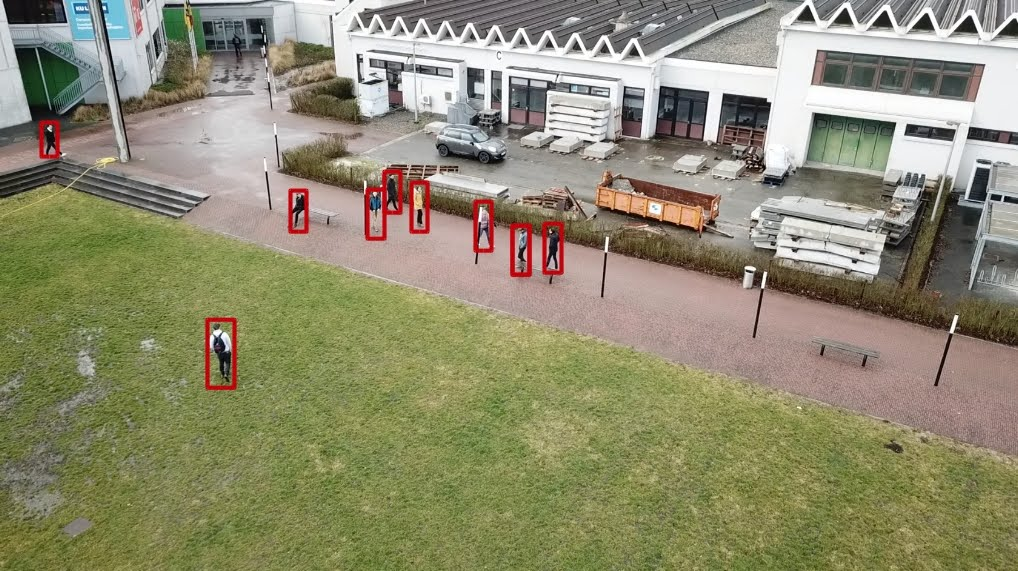
\includegraphics[width=0.56\linewidth]{3-visdrone-example}
    \caption{Примеры изображений SDD и VisDrone наборов данных} \label{sdd-visdrone-example}
\end{figure}


В силу специфичности решаемой задачи, пришлось самостоятельно формировать и организовывать сбор обучающей выборки с необходимыми нам фотографиями. Для решения этой задачи были привлечены добровольцы из различных ПСО, а также, разработаны методические материалы по сбору и разметке данных \cite{lib-lacmus-wiki-images}\cite{lib-lacmus-wiki-label}.

В результате был получен уникальный в своем роде набор данных, получивший в последствии название Lacmus Drone Dataset (LaDD) \cite{lib-ladd}. LaDD состоит из 1431 фотографии и имеет формат аннотирования Pascal VOC \cite{lib-pascal} с одним классом "Pedestrian" (пешеход). Dataset также является открытым и распространяется по лицензии GNU GPL v3. В его создании приняло участие множество ПСО из различных регионов России (Москва, Саратов, Ямал, Крым, Калининград и др). Таким образом, удалось достичь высокого разнообразия природных условий и, как следствие, и обучающей выборки. Ниже приведен пример фотографии:

\addimghere{3-ladd-example}{1}{Московская область, осень 2019, бурелом, лежачий на боку человек}{ladd-example}

\clearpage % Постановка задачи
%\input{inc/0-conclusion} % Заключение
%\input{inc/0-bibliography} % Библиографический список

% Приложения
%\vspace*{\fill}
\centering{\uppercase{Приложение}}
\vspace*{\fill}

\clearpage

\appsection{Приложение А}
\centering{\uppercase{Исходный код интерфейсов системы модулей и модуля LacmusRetinanetPlugin.DirectML}}
\vspace{\baselineskip}

\lstinputlisting[numbers=left]{inc/scripts/lacmus-plugins/LacmusPlugin/IObjectDetectionPlugin.cs}

\lstinputlisting[numbers=left]{inc/scripts/lacmus-plugins/LacmusPlugin/IObjectDetectionModel.cs}

\lstinputlisting[numbers=left]{inc/scripts/lacmus-plugins/LacmusPlugin/IObject.cs}

\lstinputlisting[numbers=left]{inc/scripts/lacmus-plugins/LacmusPlugin/Version.cs}

\lstinputlisting[numbers=left]{inc/scripts/lacmus-plugins/LacmusPlugin/Enums/InferenceType.cs}

\lstinputlisting[numbers=left]{inc/scripts/lacmus-plugins/LacmusPlugin/Enums/OperatingSystem.cs}

\lstinputlisting[numbers=left]{inc/scripts/lacmus-plugins/LacmusRetinanetPlugin.DirectML/Model.cs}

\lstinputlisting[numbers=left]{inc/scripts/lacmus-plugins/LacmusRetinanetPlugin.DirectML/Plugin.cs}

\clearpage % Исходный код скрипта DDoS Deflate
%\input{inc/b-app} % Руководство пользователя

%\includepdf{act} % Акт внедрения

\end{document}
%%% Конец документа